\chapter{\label{ch:experiments}Experiments}
In this chapter, we will describe the experiments we made and present the
results we obtained. In Section~\ref{sec:clone-detection-experiments}, we will
present our experiments about code clone detection, while in
Section~\ref{sec:token-generation-experiments} we will describe our experiments
to generate token embedding. In both sections we will show what kind of data we
used to train our model and how our model perform with different
hyper-parameters.
\section{\label{sec:clone-detection-experiments}Code clone detection}
To evaluate our clone detection model, we implemented the model we described
in~\ref{sec:clone-detection}, we collected data of programs implementing the
same functionality to feed to the model, and we trained and evaluated our model
with different hyper-parameters. In this section, we will give some details
about the data we collected for our experiments and present the different
results we obtained when evaluating our model.
\subsection{\label{ssec:clone-detection-dataset}Code clone detection dataset}
As we are using a supervised learning approach to code clone detection, to train
our model we needed data which fulfills the following properties.

\begin{enumerate}
\item Multiple code fragments should implement the same functionality
\item Information on whether two code fragments implement the same functionality
  must be included
\item Dataset should contain code fragments written in at least 2 programming
  languages
\end{enumerate}

To the best of our knowledge, no dataset currently available fulfills all the
necessary properties to our experiments, therefore we created our own dataset.

For this dataset, we found that competitive programming websites are an
excellent match. The solution to a single problem is implemented by a
large number of persons in many different languages. All the solutions to a
single problem must implement exactly the same functionality, therefore,
we are assured that all source codes implementing a solution to the same problem
are at least type IV code clones. The easier the problem is, the higher the
probability of code fragments implementing the solution to the same problem have
to be very similar to each other, and to therefore be closer to type III clones.
Furthermore, multiple solutions to a problem are always implemented by different
users, which makes our dataset closer to the motivating example we presented in
Section~\ref{sec:motivating-exmaple}.

To create the dataset, we scraped code from a famous Japanese competitive
programming website. As our implementation currently only supports Java and
Python, we fetched data for these two programming languages. We restricted the
data to only programs that were accepted by the website judging system --- meaning
that the programs actually implemented the solution to the given problem --- in
order to have the type IV code clone guarantee. In
table~\ref{tab:clone-dataset-overview}, we give some statistics about the
dataset we created and in table~\ref{tab:clone-dataset-languages} we show how
the given statistics are distributed between Python and Java. We show the
distribution of the number of files per problem --- which is representative of
the number of clones in the dataset --- in
figure~\ref{fig:files-per-problem-distribution}.

\begin{table}
  \caption{\label{tab:clone-dataset-overview} Clone detection dataset overview}
  \begin{center}
    \begin{tabular}{c c}
      Statistic & Value\\
      \toprule
      Problems count & 576\\
      Avg. files / problem & 77\\
      Files count & 44620\\
      Lines count & 1270599\\
      Tokens count & 8554476
    \end{tabular}
  \end{center}
\end{table}

\begin{table}
  \caption{\label{tab:clone-dataset-languages} Clone detection dataset language overview}
  \begin{center}
    \begin{tabular}{c c c}
      & Python & Java\\
      \toprule
      Avg. files / problem & 41 & 36\\
      Files count & 23792 & 20828\\
      Lines count & 312353 & 958246\\
      Tokens count & 1810085 & 6744391
    \end{tabular}
  \end{center}
\end{table}

\begin{figure}
  \begin{center}
    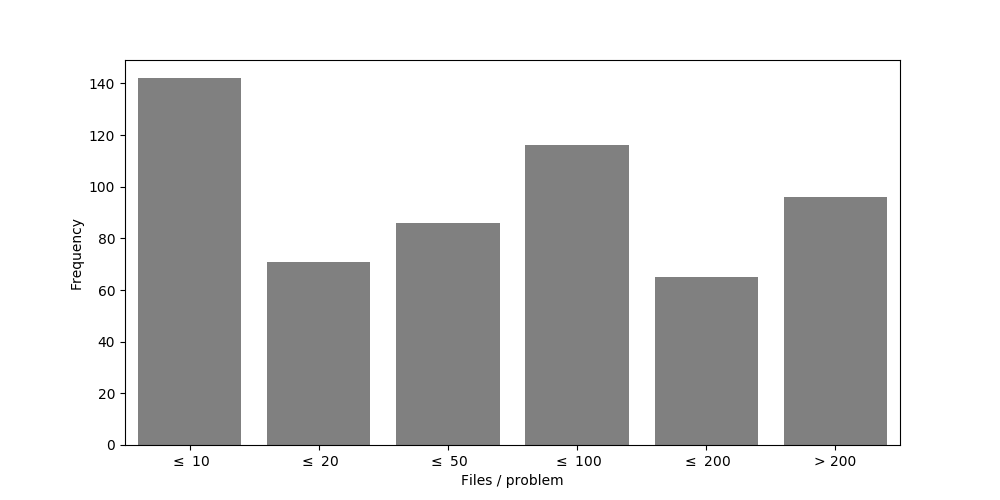
\includegraphics[width=17cm]{./images/code-clone-dataset-problems-distribution.png}
    \caption{\label{fig:files-per-problem-distribution} Distribution of the
      number of files per problem}
  \end{center}
\end{figure}

In order to be able to feed the code to our model, we transform the code we
fetched using \lstinline{bigcode-astgen} we presented in
Section~\ref{sec:ast-generation}.
\section{\label{sec:token-generation-experiments}Token embedding generation}
